\section{Discontinuous Galerkin method}

For complex problems of compressible flow, and of course for even more complex problems of compressible MHD, there has been a number of attempts to use standard and well known Finite Element Methods that replace the spaces defined in \cref{Bochner} with finite-dimension spaces with bases formed by continuous piecewise polynomial functions. These attempts struggled with a common problem of spurious oscillations appearing in the solution - the origin of which is the lack of "stabilization", provided by the second-order terms in elliptic equations. Solution to these problems is the application of stabilization techniques, that usually introduce some sort of artificial diffusion (the second-order term), all of which are non-physical, and generally involve "magical" numbers - constants that are of pure computational nature (not a part of the physical description) or even worse are problem-specific.

\subsection{Overview of the DG method}
Due to this reason, there  was an effort to develop methods which would not need such stabilization techniques, and would still offer reasonable resolution of shockwaves, boundary and interior layers, and steep gradients without exhibiting spurious oscillations in the approximate solutions. The approach taken here is based on the idea to combine finite volume and Finite element methods leading to the so-called \emph{discontinuous Galerkin finite element method (DGFEM, DG)}. Here we shall derive and analyze DG for our equations. Let $T_h$ be a triangulation of $\Omega$.
By $H^1\lo\Omega, T_h\ro$ we denote the so-called \textit{broken Sobolev space}:
\be
\label{BrokenSobolev} H^1\lo\Omega,T_h\ro = \left\{v\in L^2\lo\Omega\ro;\ v|_K\in H^1\lo K\ro \forall K\in T_h\right\}.
\ee
This space is an approximation of the space defined in \cref{Sobolev}, but it contains functions that are discontinuous on element interfaces $\Gamma_{ij}$ between elements $K^i and K^j$.
\paragraph{}
For $u\in H^1\lo\Omega,T_h\ro$ we set
\be
\label{PlusDef} u_K^i = \text{trace of } u|_{K^i} \text{ on }\partial K^i
\ee
(i.e. the interior trace of $u$ on $\partial K^i$). For each face $\Gamma_{ij}\subset\partial K\backslash\Gamma$ of $K^i$, there exists $K^j\neq K^i,\ K^j\in T_h$, adjacent to $\Gamma_{ij}$ from the opposite side than $K^i$. Then we put
\be
\label{MinusDef} u_K^j = \text{trace of } u|_{K^j} \text{ on } \Gamma_{ij}.
\ee
In this way we obtain the exterior trace $u_K^j$ of $u$ on $\partial K^i\backslash\Gamma$ and define the jump of $u$ on $\partial K\backslash\Gamma$:
\be
[u]_{\Gamma_{ij}} = u_K^i - u_K^j.
\ee
\subsubsection{Approximation of the broken Sobolev space}
\label{section:Vh}
Let the domain $\Omega$ be covered with a mesh $T_h = 
\{ K_1,$ $K_2, \dots, K_M \}$ where each element $K_m$ carries an arbitrary
polynomial degree $1 \leq p_m$, $\forall m = 1, 2, \dots, M$. The broken Sobolev space 
$H^1\lo\Omega,T_h\ro$ will be approximated by a finite-dimensional space of piecewise-polynomial functions
\be
\label{VH} V_{h} = \{ v \in L^2(\Omega); \ v|_{K_m} \in P^{p_m}(K_m)\ \mbox{for all}\ 1 \leq m \leq M \}
\ee
where $P^{p}$ is defined as
\bd
P^{p} = \mbox{span}\{\sum_{\substack{0\leq i, j, k \leq p \\i+j+k\leq p}}\alpha_i\ x_1^i\ x_2^j\ x_3^k,\ \ \alpha_i\in\mathbb{R} \}.
\ed

\subsection{DG formulation of MHD equations}
Although the resulting system will look very similar to the weak formulation \cref{WeakFinal}, the derivation makes more sense to be done starting with the \cref{conservativeGeneric}.
\paragraph{}
As stated in \cref{section:triangulation}, at this point we will discretize the problem in space, and leave the time-derivative untouched.
The approximate solution will be sought at each time instant $t$ as an element of the finite-dimensional space
\be
\label{feSpaceDef}
\left[V_h\right]^8,
\ee
where $V_h$ is defined in \cref{VH}. Functions
\be
\label{feSpaceBasis}
\mrvh \in \left[V_h\right]^8\approx \left[H^1\lo\Omega,T_h\ro\right]^8,
\ee
where $H^1\lo\Omega,T_h\ro$ is defined in \cref{BrokenSobolev}, are in general discontinuous on interfaces $\Gamma_{ij}$.
By $\mrvh|_{ij}$ and $\mrvh|_{ji}$ we denote the values of $\mrvh$ on $\Gamma_{ij}$ considered from the
interior and the exterior of $K^i$, respectively. The symbols
$$
\left<\mrvh\right>_{ij} = \frac12 \lo \mrvh |_{ij} + \mrvh |_{ji}\ro,\ \left[\mrvh\right]_{ij} = \mrvh |_{ij} - \mrvh |_{ji}
$$
denote the average and jump of a function $\mrvh$ on $\Gamma_{ij}$.
In order to derive the discrete problem, we multiply \cref{conservativeGeneric} by a test function $\mrvh \in \left[V_h\right]^8$ in a component-wise fashion, integrate over any element $K^i \in T_h$, apply Green's theorem and sum over all $i \in I$, where $I$ is defined in \cref{Idef}:
\be
\label{DG1} \int_{\Omega_{t}} \pds{{\mrPsi_h}}{t} \mrvh - \sum_{K^i \in T_h}\int_{K^i}\mrF\lo{\mrPsi_h}\ro \lo\nabla \cdot \mrvh\ro + \sum_{K^i\in T_h} \sum_{j\in s_i} \int_{\Gamma_{ij}} \lo \mrF\lo{\mrPsi_h}\ro \cdot \bfn_{ij} \ro \mrvh = \int_{\Omega_{t}} \mrS \mrvh,
\ee
where $\bfn_{ij}$ is the unit outer normal to $\Gamma_{ij}$.
Now, the term
\be
\label{NonUniqueTerm} \int_{\Gamma_{ij}} \mrF\lo{\mrPsi_h}\ro \cdot \bfn_{ij} \mrvh
\ee
is problematic, because the value of ${\mrPsi_h}$ on $\Gamma_{ij}$ is not unique - we have two values:
\begin{itemize}
    \item ${\mrPsi_h}|_{ij}$ - which is the value of ${\mrPsi_h}$ on $\Gamma_{ij}$ considered from the element $K^i$,
    \item ${\mrPsi_h}|_{ji}$ - which is the value of ${\mrPsi_h}$ on $\Gamma_{ij}$ considered from the element $K^j$.
\end{itemize}
\textbf{Note: }This corresponds to the notation set in \cref{PlusDef,MinusDef} - if we take $K^i$ as the element at hand, we have
$$
{\mrPsi_h}|_{ij} = {\mrPsi_h}_{K^i}^+,\ \ {\mrPsi_h}|_{ji} = {\mrPsi_h}_{K^i}^-
$$
\paragraph{}
Now, because of this non-uniqueness of the values, we replace the term \cref{NonUniqueTerm} with the so-called \textit{numerical flux} $\mrH = \mrH\lo\mrv, \mrw, \bfn\ro$ in the following fashion:
\be
\label{NumFluxDef}
\lo\mrF\lo{\mrPsi_h}\ro \cdot \bfn_{ij}\ro \mrvh \approx \mrH\lo{\mrPsi_h}|_{ij}, {\mrPsi_h}|_{ji}, \bfn_{ij}\ro \mrvh.
\ee
We impose the following requirements on the numerical flux:
\begin{enumerate}
	\item $\mrH\lo \mrv, \mrw, \bfn\ro$ is defined and continuous on $\mc{D} \times \mc{D} \times \mc{S}_1$, where $\mc{D}$ is the domain of definition of the flux $\mrF$ and $\mc{S}_1$ is the unit sphere in $\mathbb{R}^3$.
	\item $\mrH$ is $consistent$:
		\be
			\label{FluxConsistent} \mrH\lo \mrv, \mrv, \bfn\ro = \mrF\lo \mrv\ro \bfn,\ \mrv\in\mc{D},\ \bfn\in\mc{S}_1.
		\ee
	\item $\mrH$ is $conservative$:
		\be
			\label{FluxConservative} \mrH\lo \mrv, \mrw, \bfn\ro = -\mrH\lo \mrw, \mrv, -\bfn\ro,\ \mrv, \mrw\in\mc{D},\ \bfn\in\mc{S}_1.
		\ee
 \end{enumerate}

And using these properties of the numerical flux, we can rewrite \cref{DG1} as:
\begin{align}
    \label{DG2} \int_{\Omega_{t}} \pds{{\mrPsi_h}}{t} \mrvh & - \sum_{K^i \in T_h}\int_{K^i}\mrF\lo{\mrPsi_h}\ro \lo\nabla \cdot \mrvh\ro\\
    \nonumber & + \sum_{\Gamma_{ij}\in\Gamma_I} \int_{\Gamma_{ij}} \mrH\lo{\mrPsi_h}|_{ij}, {\mrPsi_h}|_{ji}, \bfn_{ij}\ro \mrvh = \int_{\Omega_{t}} \mrS \mrvh,
\end{align}
where we used the definition of internal edges (\cref{InternalEdges}).
\subsection{Numerical flux}
Generally, the numerical flux function can be a non-differentiable (or even discontinuous) function. That renders it impossible to directly employ Newton's method to solve the resulting nonlinear problem, and either linearization (e.g. a semi-implicit scheme - \cite{dolejsi2015}, chapter 5.1) or explicit time discretization (used in this work) needs to be used.
\paragraph{}
Another complication arising from evaluation of numerical fluxes on element interfaces exists in distributed solver, where we need to make sure that all processors have relevant data (e.g. previous solution values) from all cells that neighbor any cells assembled on the processor at hand. This issue gets worse when local mesh refinement (there are more neighbor elements of the current cell across the interface at hand), as well as if periodic boundary conditions are used (the neighbor graph is more complex).
\subsubsection{Lax-Friedrichs numerical flux}
This is the most straightforward numerical flux satisfying \cref{FluxConsistent}, and \cref{FluxConservative} and is defined as follows:
\be
\mrH_{LF}\lo \mrv, \mrw, \bfn\ro = \frac12\left[\mrF\lo\mrv\ro + \mrF\lo\mrw\ro\right] - \frac{\alpha}{2}\lo \mrw - \mrv\ro,
\ee
where the parameter $\alpha$ is the so-called \textit{stabilization parameter}, which in order for the solution to be stable needs to fulfill $\alpha < \frac{\Delta t}{\Delta x}$, where $\Delta t, \Delta x$ need to satisfy the CFL condition \cref{equation:CFLcond}. Now, this numerical flux is very sensitive to the choice of $\alpha$ - for larger values, it tends to be very diffusive, but for lower values, it is unstable and produces oscillations in the vicinity of shocks \cite{lfunstable}. In this work it is primarily used for implementation verification purposes, as due to its simplicity, the risk of errors in its implementation is rather negligible.

\subsubsection{Riemann problem for MHD}
For the class of numerical fluxes, known as the \textit{Godunov type fluxes}, the numerical flux across the element boundary is constructed as the flux $\mrF$ of a solution of the following Riemann problem (\cref{Riemann}) at $x = 0$:
\be
\label{Riemann}
\frac{\partial \mrU}{\partial t} + \frac{\partial \mrF}{\partial x} = 0,
\ee
where
\begin{align}
\label{RiemannUDef}
\mrU & =  \lo\begin{array}{c}\rho \\ \pi_1 \\ \pi_2 \\ \pi_3 \\ U \\ B_2 \\ B_3 \\ \end{array}\ro,\ \mrF = \lo\begin{array}{c} \pi_1 \\ \frac{\pi_1^2}{\rho} - B_1^2 + \frac12\lo p + U_m\ro \\ \frac{\pi_2 \pi_1}{\rho} - B_1 B_2 \\ \frac{\pi_3 \pi_1}{\rho} - B_1 B_3\\ \frac{\pi_1}{\rho} \lo \frac{\gamma}{\gamma - 1} p + U_k\ro + \frac{2}{\rho} \lo \pi_k B_1 - \pi_1 B_k\ro B_1  \\ \frac{\pi_1 B_2 - \pi_2 B_1}{\rho} \\ \frac{\pi_1 B_3 - \pi_3 B_1}{\rho} \\ \end{array}\ro,
\end{align}
with two states
\begin{align}
\mrU_L & =  \lo\rho_L, {\pi_1}_L, {\pi_2}_L, {\pi_3}_L, {U}_L, {B_2}_L, {B_3}_L \ro
\mrU_R & =  \lo\rho_R, {\pi_1}_R, {\pi_2}_R, {\pi_3}_R, {U}_R, {B_2}_R, {B_3}_R \ro,
\end{align}
and where due to the divergence free condition $\nabla\cdot \bfB = 0$ of the magnetic field), $B_1$ is given as constant.
\paragraph{}
These equations (\cref{Riemann}) have seven eigenvalues which correspond to two Alfve'n waves ($\lambda_{2, 6}$), two slow magneto-acoustic waves ($\lambda_{3, 5}$), and two fast magneto-acoustic waves ($\lambda_{1, 7}$), and one entropy wave ($\lambda_{4}$):
\begin{align}
\lambda_{1} = \bfu_x - c_f,\\
\lambda_{2} = \bfu_x - c_a,\\
\lambda_{3} = \bfu_x - c_s,\\
\lambda_{4} = \bfu_x,\\
\lambda_{5} = \bfu_x + c_s,\\
\lambda_{6} = \bfu_x + c_a,\\
\lambda_{7} = \bfu_x + c_f,
\end{align}
where $c_a = \sqrt{\frac{B_1^2}{rho}}$, $c_{s, f} = \left\{\frac{\gamma p + |B|^2 \mp \sqrt{\left(\gamma p + |B|^2\right)^{\frac12} - 4\gamma p B_1^2}}{2\rho}\right\}^{\frac12}$.
\paragraph{}
From this, it follows, that there are theoretically as many as 9 states (states between the characteristics equal to the eigenvalues $\lambda_1, ..., \lambda_7$ along which the solution propagates) - see \cref{figure:allRiemannStates}.

\begin{figure}[H]
	\centering
		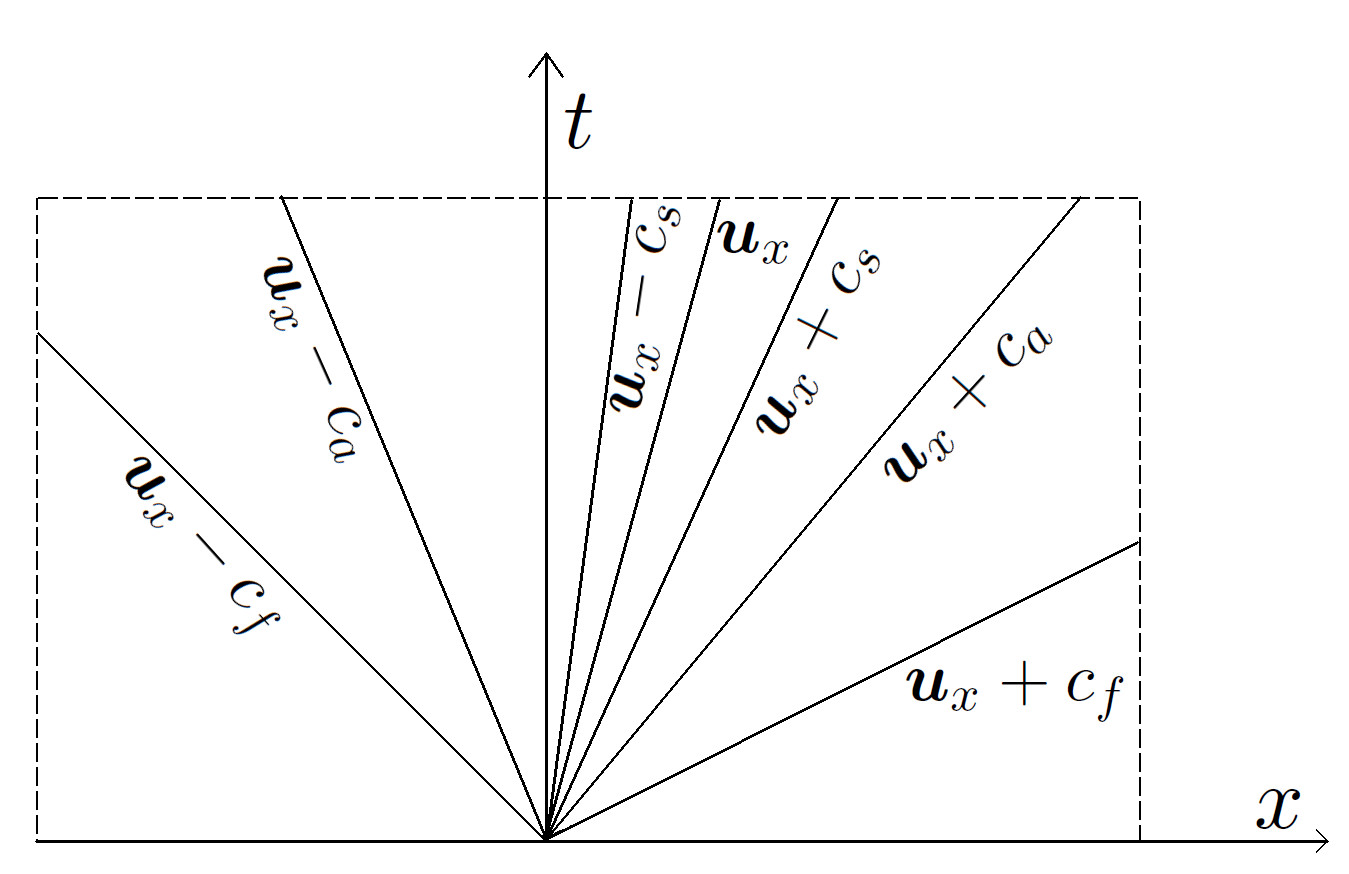
\includegraphics[width=0.4\textwidth]{img/riemann/allStates.jpg}
		\vspace{-3mm}
	\caption{Characteristics corresponding to eigenvalues of \cref{Riemann}.}
	\label{figure:allRiemannStates}
\end{figure}

Unfortunately, for MHD equations, there is no exact solver of the Riemann problem across the element boundary, and therefore, approximate solvers are used. One instance of the derived numerical flux based on the solution at $x = 0$ of \cref{Riemann} is described in the next section.

\subsubsection{HLLD numerical flux}
The abbreviation \textbf{HLLD} stands for Harten-Lax-van Leer (HLL) approximate Riemann solver, and \textbf{D} stands for Discontinuities. It is an extension of HLLC Riemann solver for the Euler equations (\cite{hllc}). It divides the Riemann fan into 6 states as illustrated in \cref{figure:hlldRiemannStates}. This particular numerical flux has been introduced in \cite{hlld} and has been shown to be very suitable for the studied problems. HLLD is an approximate nonlinear solution of the MHD Riemann problem, and is algebraically derived in \cite{hlld} under the assumptions that the normal velocity and the background potential magnetic field in the Riemann fan are constant. It follows from these assumptions, that 4 intermediate states are sufficient to resolve the Riemann problem in adequate manner (\cite{hlld}).

\begin{figure}[H]
	\centering
		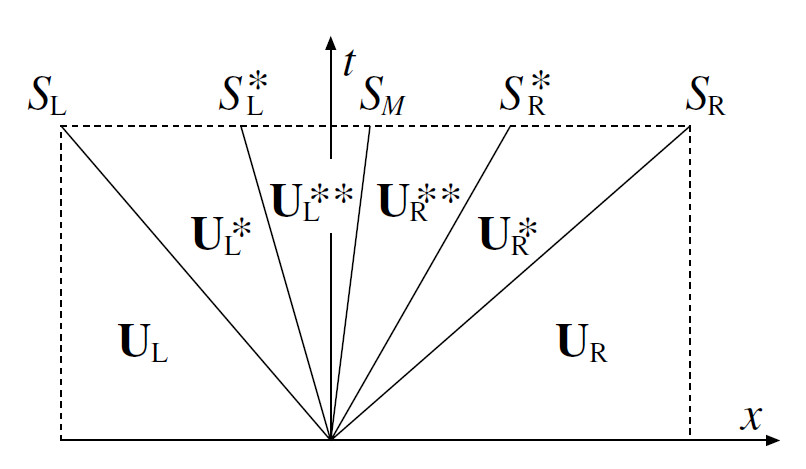
\includegraphics[width=0.4\textwidth]{img/riemann/hlldStates.jpg}
		\vspace{-3mm}
	\caption{Six states considered in the definition of HLLD flux.}
	\label{figure:hlldRiemannStates}
\end{figure}

The HLLD flux according to its definition in \cite{hlld} defines 4 intermediate (starred) states $U_L^{*}, U_L^{**}, U_R^{*}, U_R^{**}$ and 2 outer states $U_L, U_R$ corresponding to states of $U$ defined in \cref{RiemannUDef} for the left ($x < 0$) and right ($x > 0$) parts of the time-space domain illustrated in \cref{figure:hlldRiemannStates}. Details of these states are given in \cite{hlld}. The resulting fluxes are:

\be
F_{HLLD} = \left\{
	\begin{array}{l}
		F_L\ \text{if}\ S_L > 0,\\
		F^{*}_L\ \text{if}\ S_L \leq 0 \leq S_L^{*},\\
		F^{**}_L\ \text{if}\ S^{*}_L \leq 0 \leq S_M,\\
		F^{**}_R\ \text{if}\ S_M \leq 0 \leq S_R^{*},\\
		F^{*}_R\ \text{if}\ S_R^{*} \leq 0 \leq S_R,\\
		F_R\ \text{if}\ S_R < 0
	\end{array}\right. .
\ee

These are derived using the assumptions mentioned earlier, that:

\begin{align}
u^{*}_L & = u_l^{**} = u_R^{**} = u_R^{*} = S_M\ & \text{normal velocity constant over the Riemann fan}\\
p^{*}_{T_L} & = p^{**}_{T_L} = p^{**}_{T_R} = p^{*}_{T_R} = p^{*}_{T}\ & \text{total pressure constant over the Riemann fan},
\end{align}

where $p_T$ is the total pressure as defined in \cref{presT}, and

\begin{align}
S_M & \frac{\lo S_R -u_R\ro\rho_R u_R - \lo S_L - u_L\ro\rho_L u_L - p_{T_R} + p_{T_L}}{\lo S_R - u_R\ro\rho_R - \lo S_L - u_L\ro\rho_L},\\
S_L & = \mathrm{min}\left[\lambda_1\lo U_L\ro, \lambda_1\lo U_R\ro\right],\\
S_R & = \mathrm{max}\left[\lambda_7\lo U_L\ro, \lambda_7\lo U_R\ro\right],\\
S^{*}_L & = S_M - \frac{\left|B_x\right|}{\sqrt{\rho_L^{*}}} = S_M - \frac{\left|B_x\right|}{\sqrt{\rho_L\frac{S_L - u_L}{S_L - S_M}}},\\
S^{*}_R & = S_M + \frac{\left|B_x\right|}{\sqrt{\rho_R^{*}}} = S_M + \frac{\left|B_x\right|}{\sqrt{\rho_R\frac{S_R - u_R}{S_R - S_M}}}.
\end{align}


\subsubsection{Numerical fluxes comparison}
\label{subsec:numfluxcomp}
For the comparison, a simple version of the benchmark described in \cref{sec:blastNew} was used. In the next figures, there are snapshots of density solution component at several time steps for the Lax-Friedrichs flux for two values of $\alpha = 0.5,\ \alpha=1.2$, and for the HLLD flux (the higher the stabilization term $\alpha$, the more stable the scheme is). On each of \crefrange{numFluxCompare0}{numFluxCompare8}, the entire domain is shown on the left, and a plot over the line $y = 0$ is on the right.
	\begin{figure}[H]
		\begin{center}
			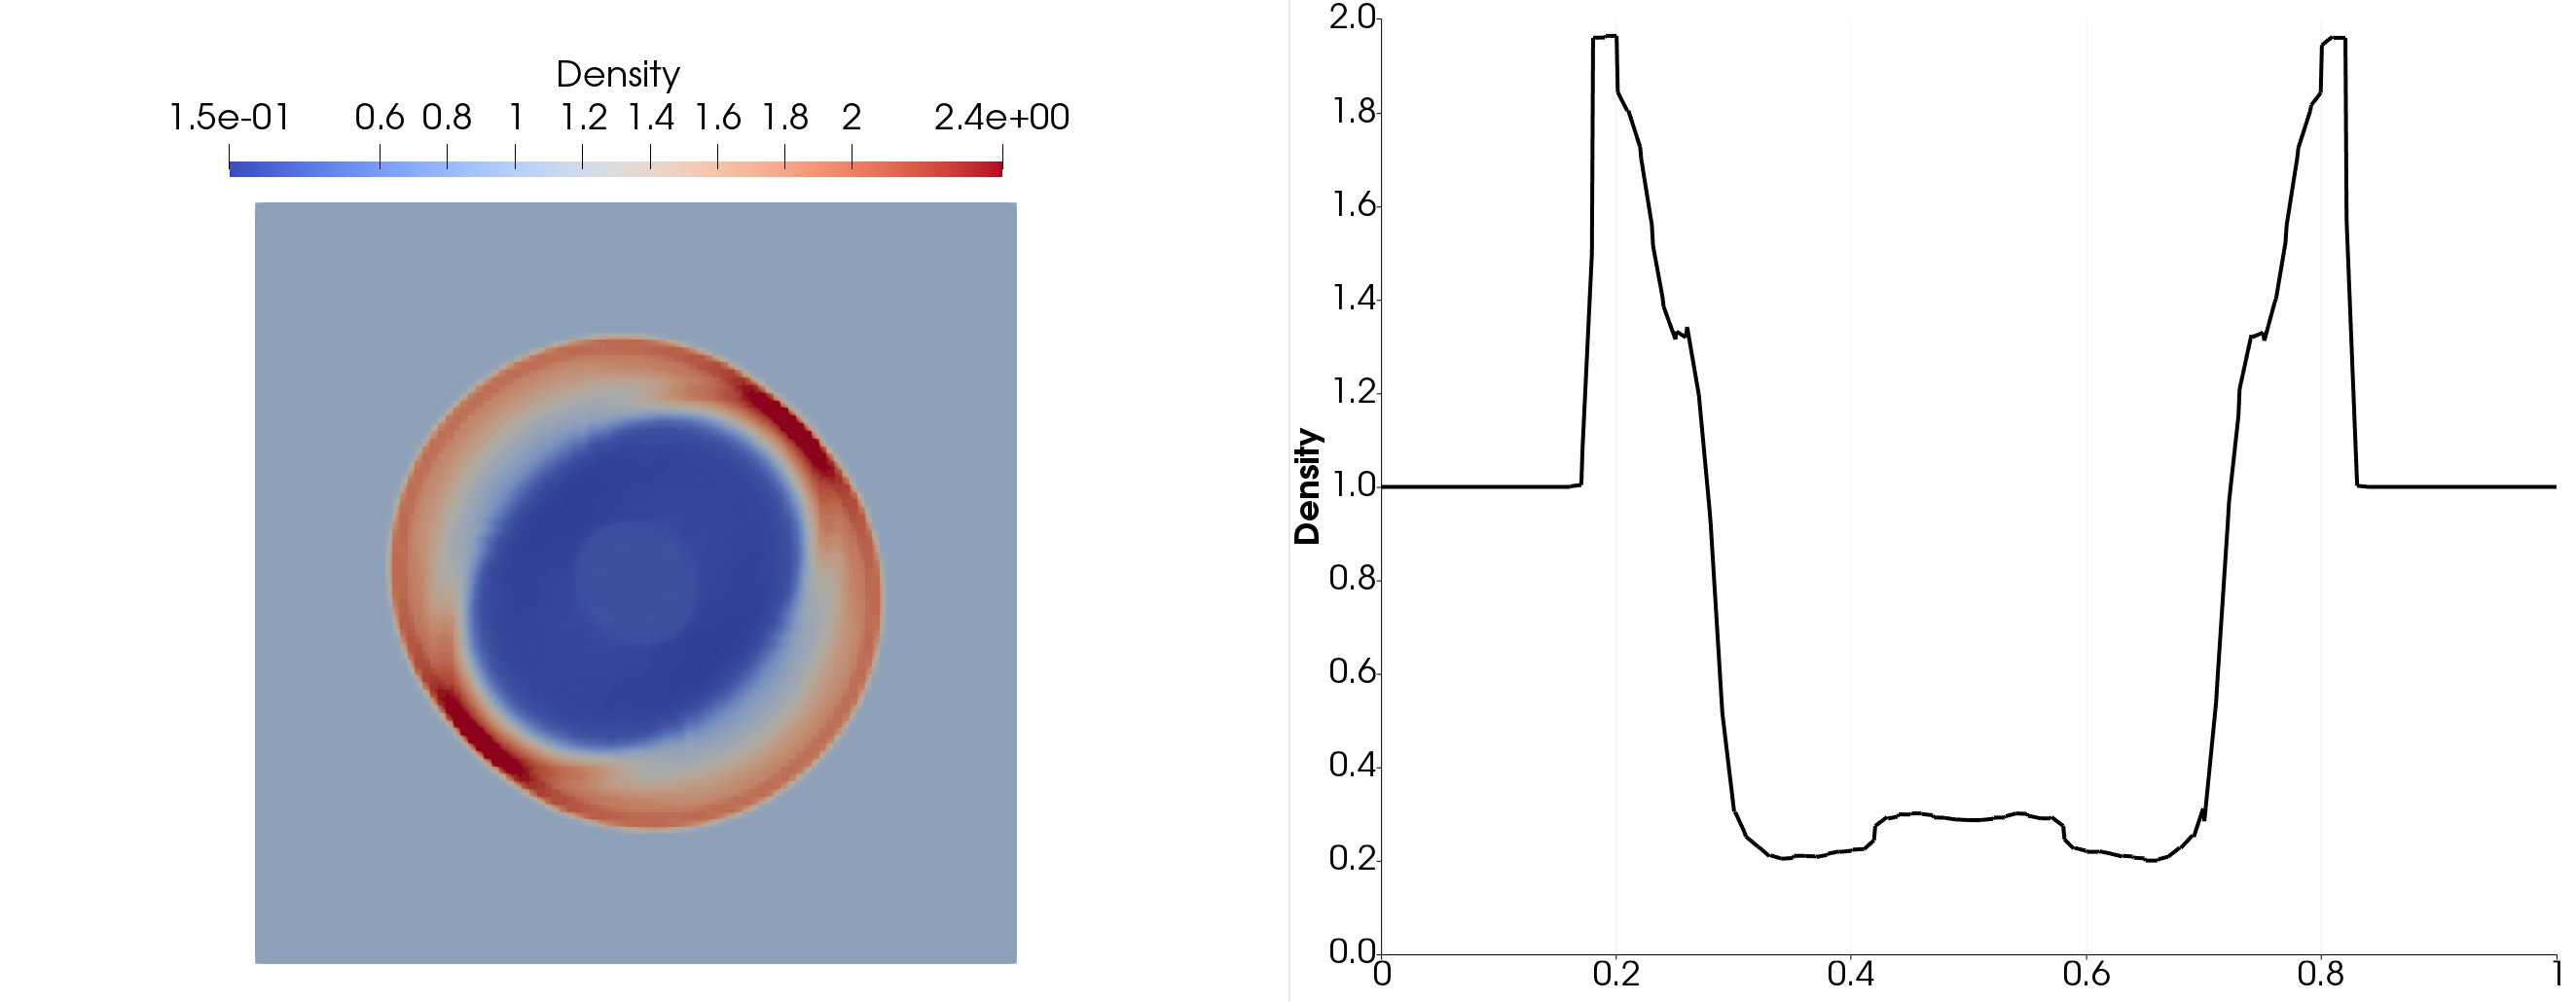
\includegraphics[width=\textwidth]{img/numflux/lf-05-0.jpg}
			\vspace{-3mm}
			\caption{Density at time $t = 0.1$, Lax-Friedrichs flux with $\alpha = 0.5$}
		\end{center}
		\label{numFluxCompare0}
	\end{figure}\vspace{-7mm}
	\begin{figure}[H]
		\begin{center}
			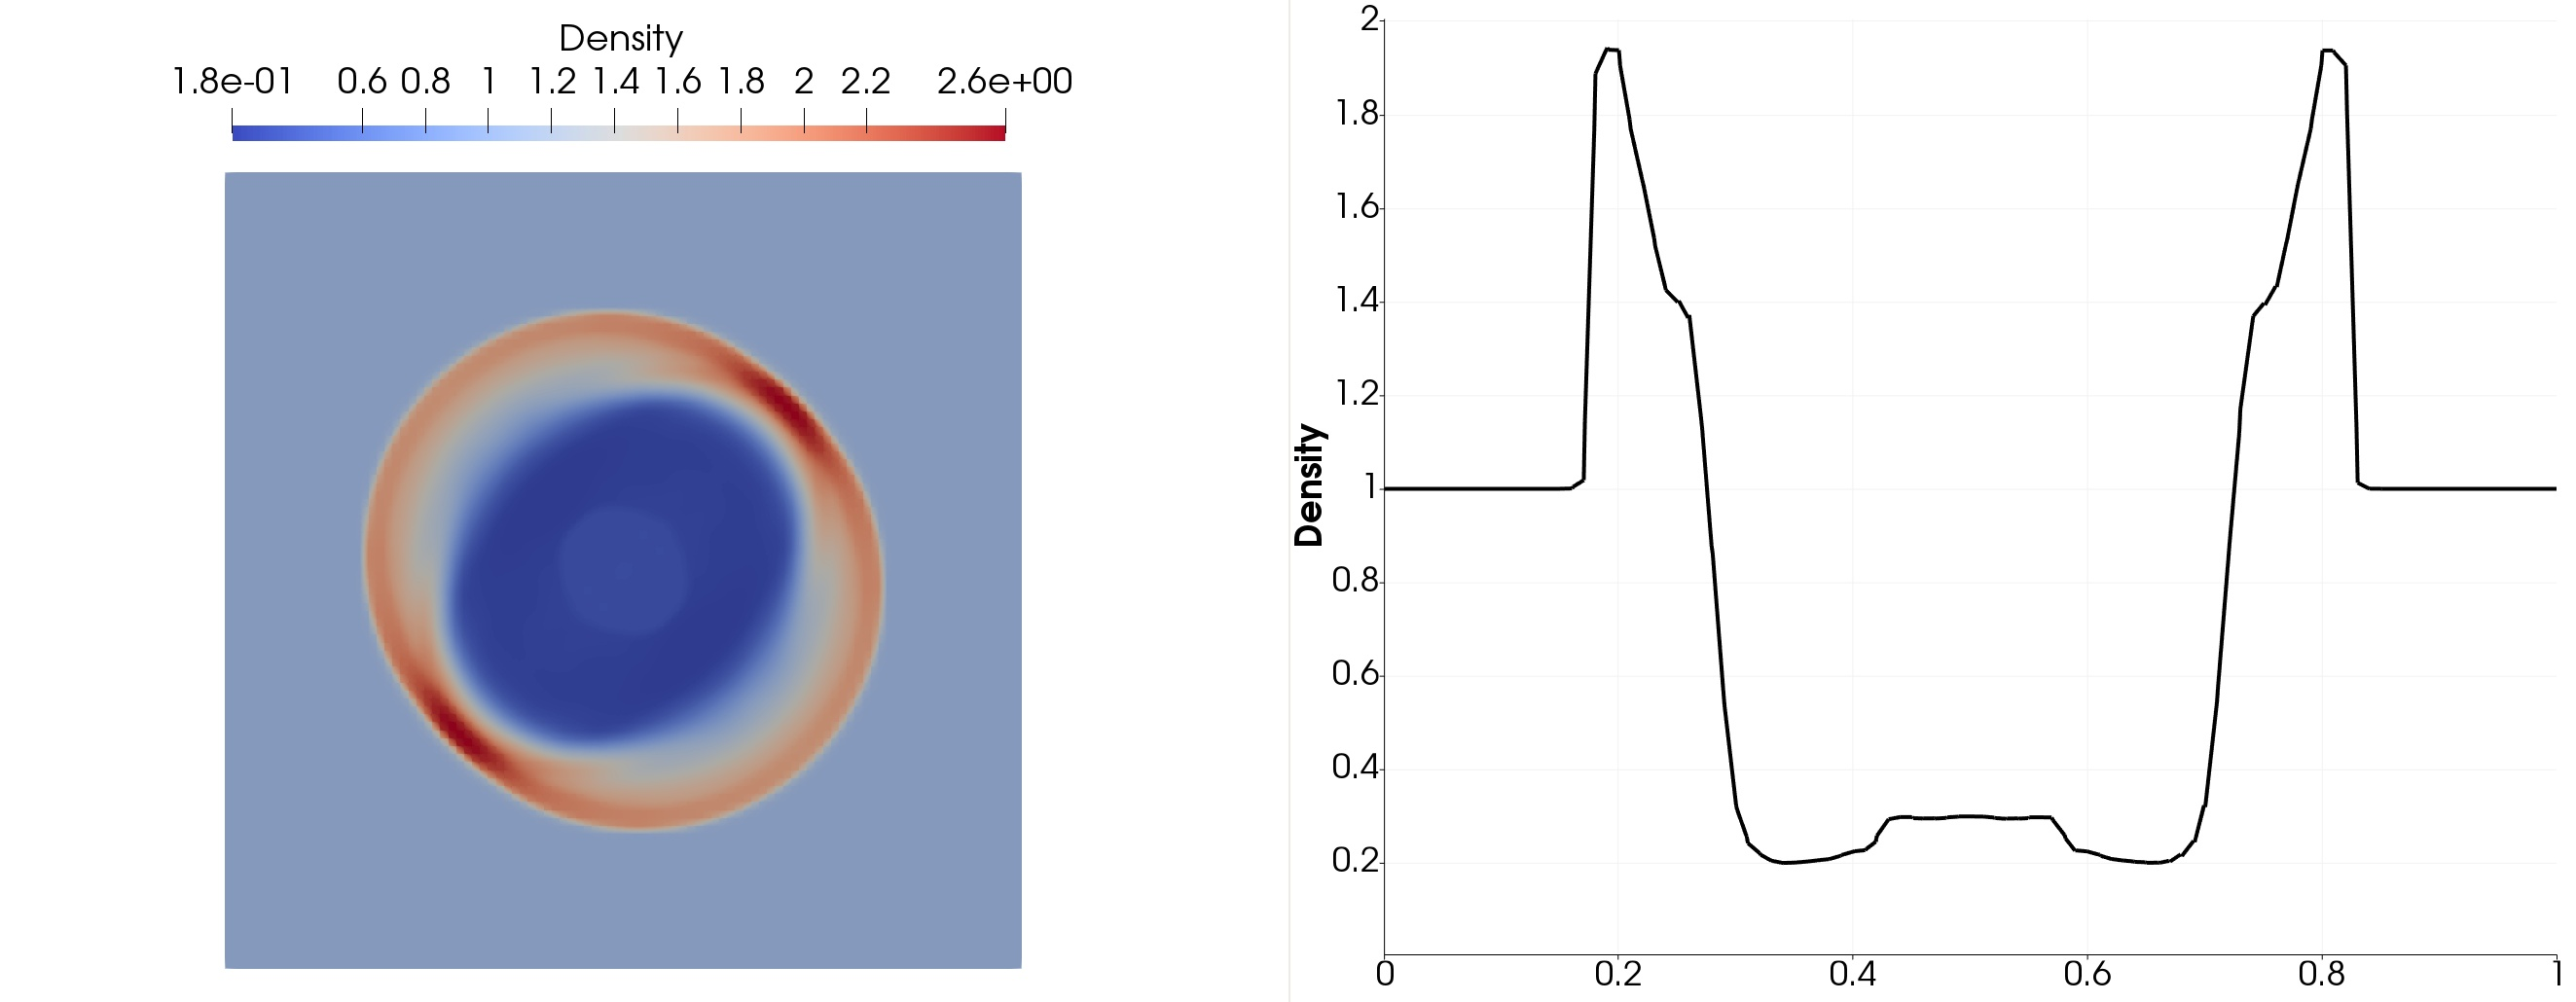
\includegraphics[width=\textwidth]{img/numflux/lf-10-0.jpg}
			\vspace{-3mm}
		\caption{Density at time $t = 0.1$, Lax-Friedrichs flux with $\alpha = 1.2$}
		\end{center}
		\label{numFluxCompare1}
	\end{figure}\vspace{-7mm}
	\begin{figure}[H]
		\begin{center}
			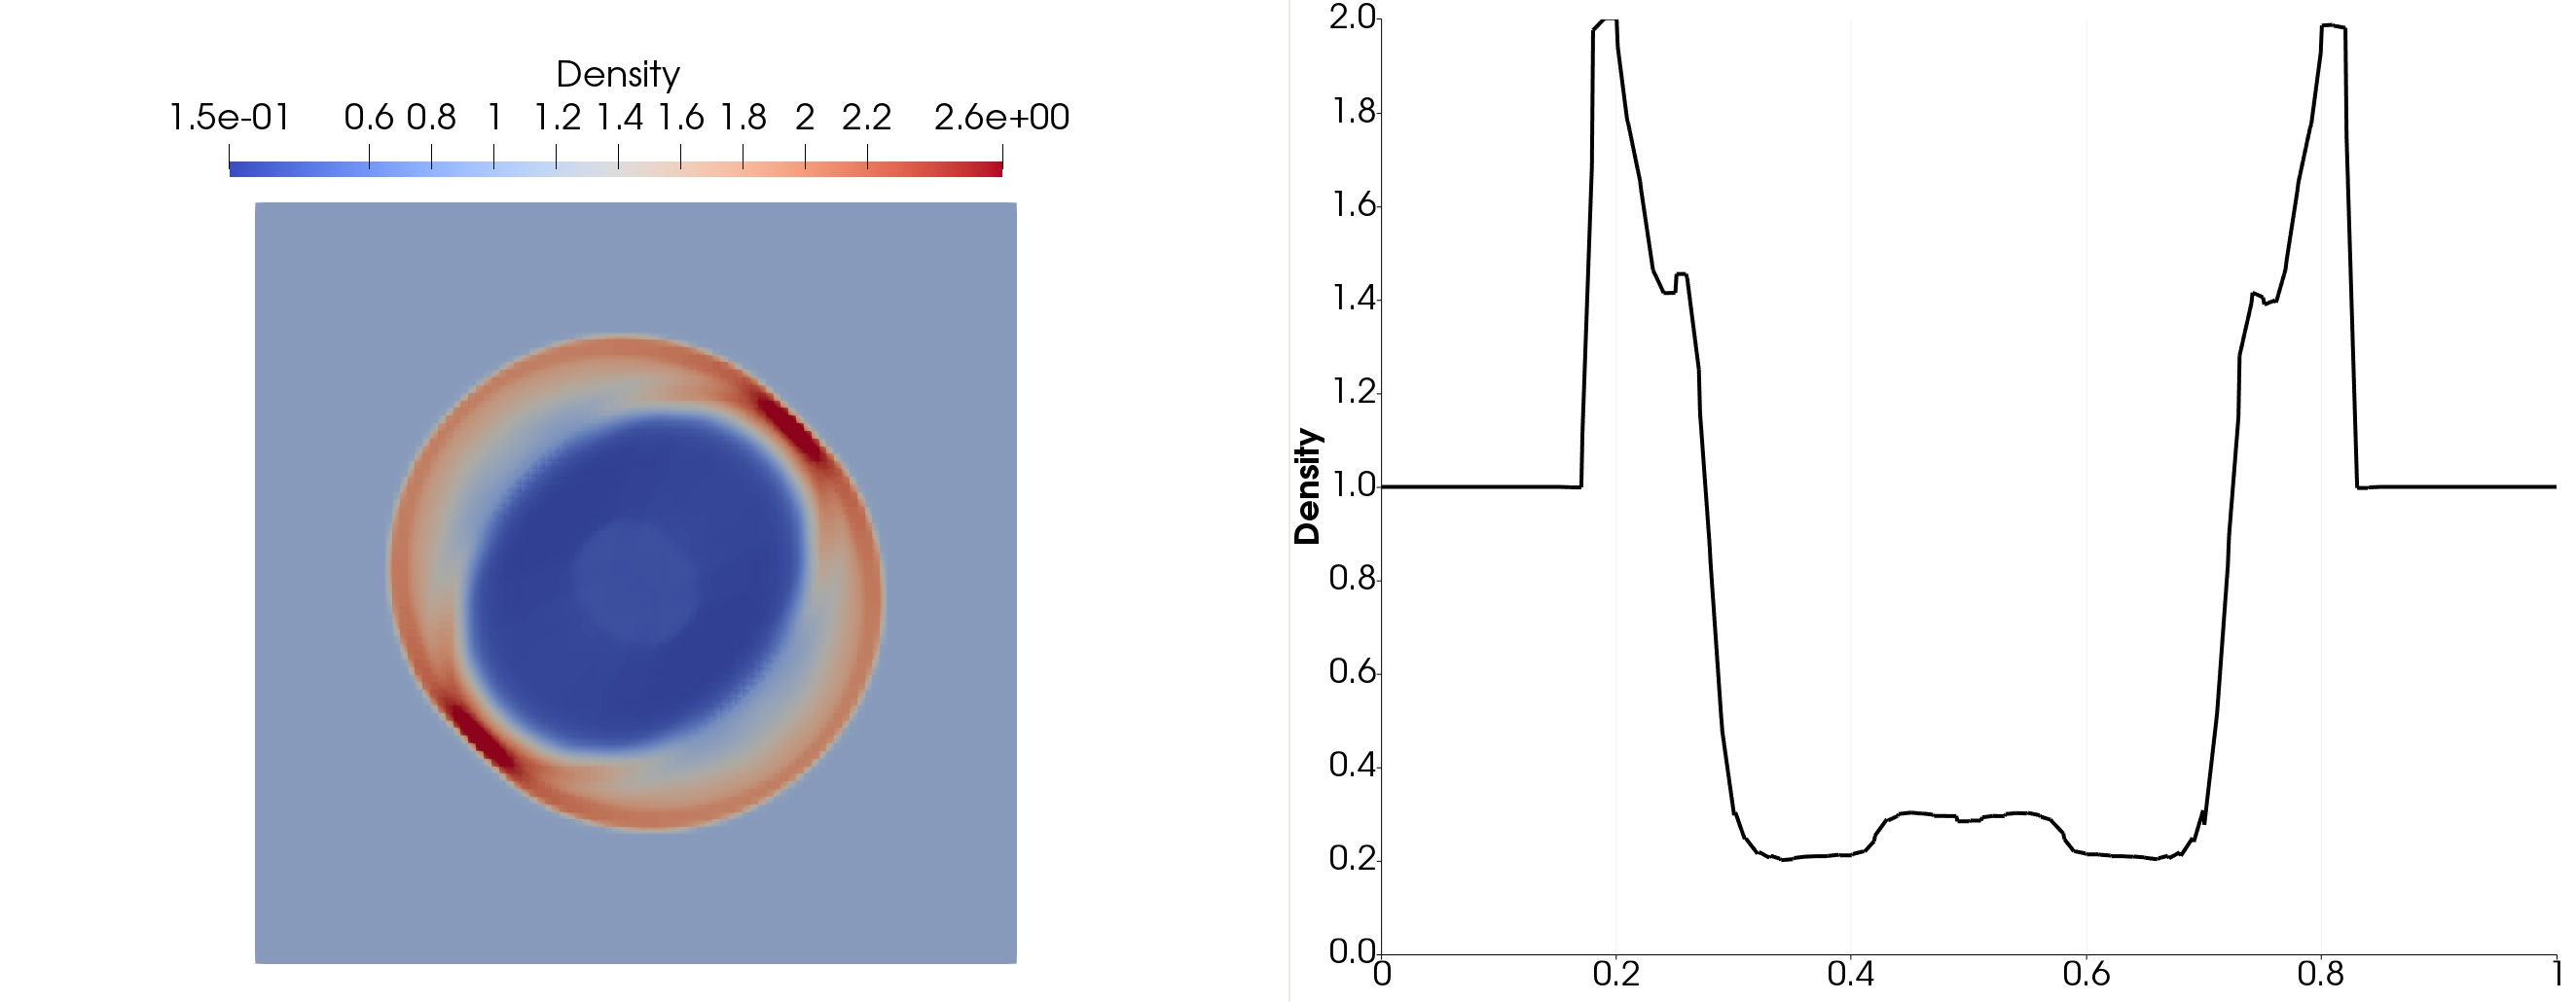
\includegraphics[width=\textwidth]{img/numflux/hl-0.jpg}
			\vspace{-3mm}
		\caption{Density at time $t = 0.1$, HLLD flux}
		\end{center}
		\label{numFluxCompare2}
	\end{figure}\vspace{-7mm}
	\newpage
	
	
	\begin{figure}[H]
		\begin{center}
			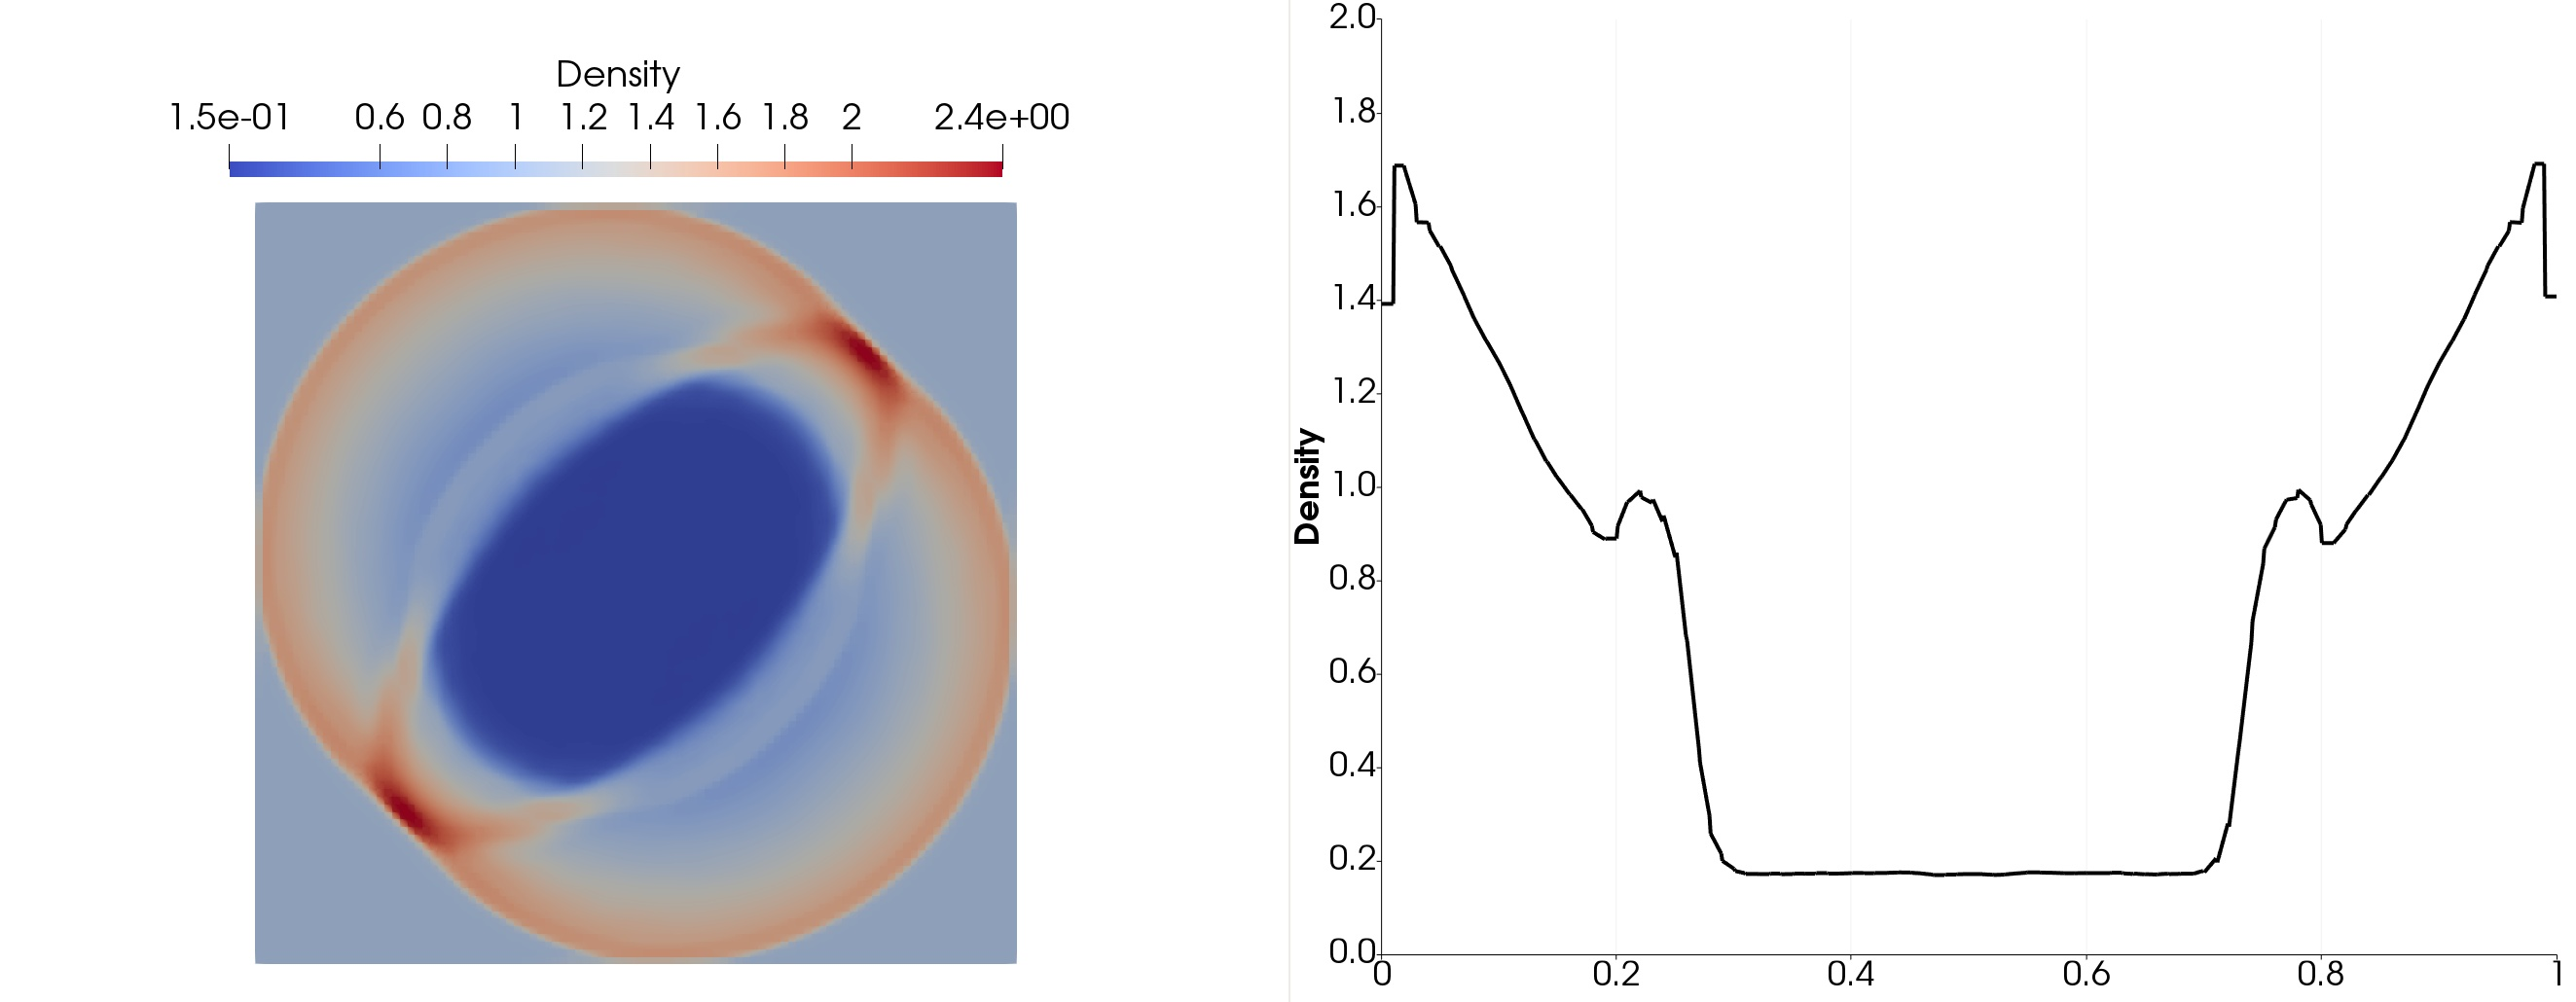
\includegraphics[width=\textwidth]{img/numflux/lf-05-1.jpg}
			\vspace{-3mm}
		\caption{Density at time $t = 0.2$, Lax-Friedrichs flux with $\alpha = 0.5$}
		\end{center}
		\label{numFluxCompare3}
	\end{figure}\vspace{-7mm}
	\begin{figure}[H]
		\begin{center}
			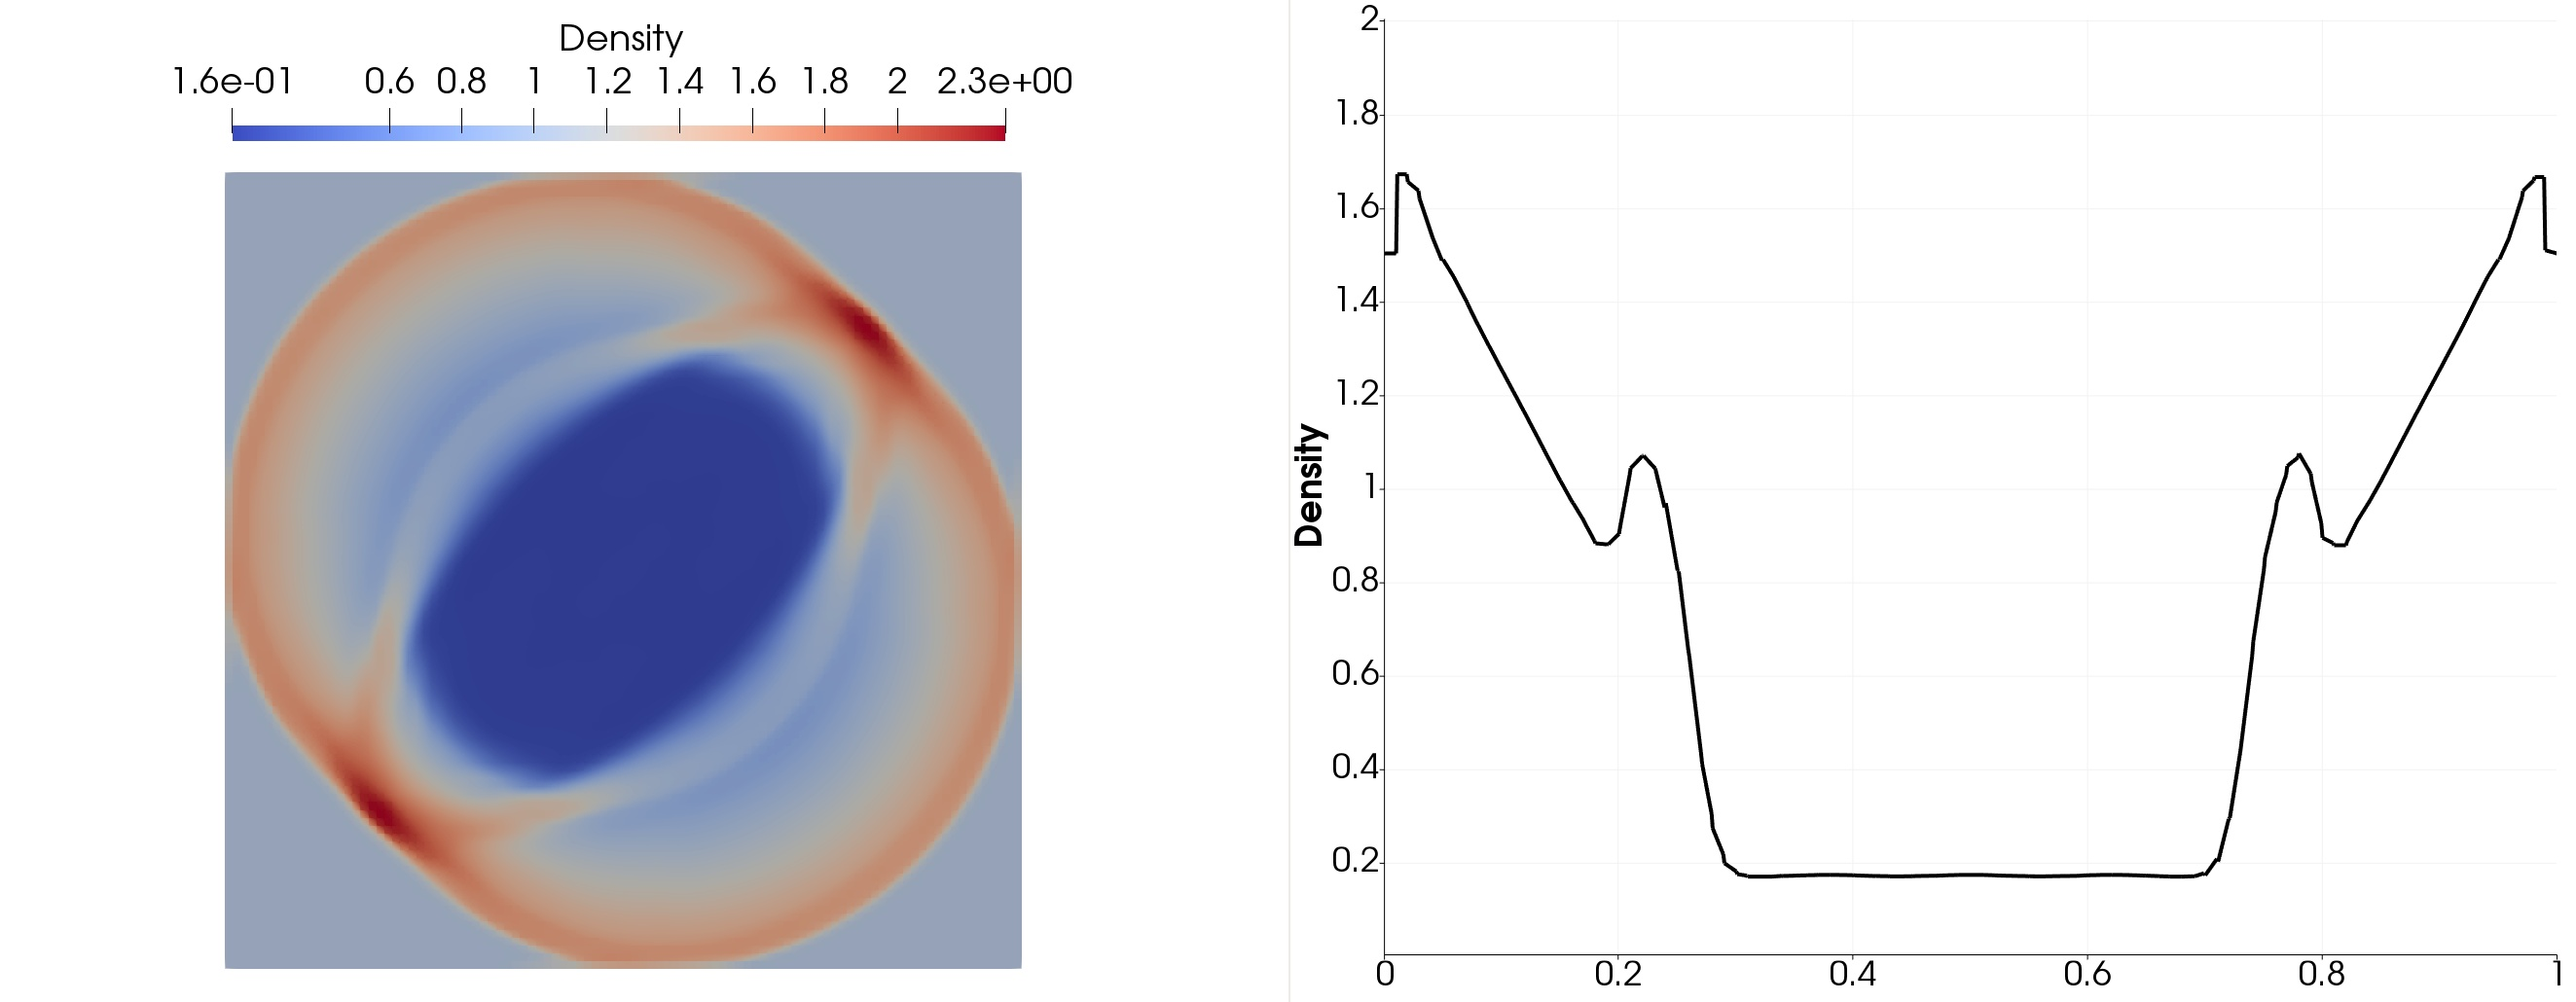
\includegraphics[width=\textwidth]{img/numflux/lf-10-1.jpg}
			\vspace{-3mm}
		\caption{Density at time $t = 0.2$, Lax-Friedrichs flux with $\alpha = 1.2$}
		\end{center}
		\label{numFluxCompare4}
	\end{figure}\vspace{-7mm}
	\begin{figure}[H]
		\begin{center}
			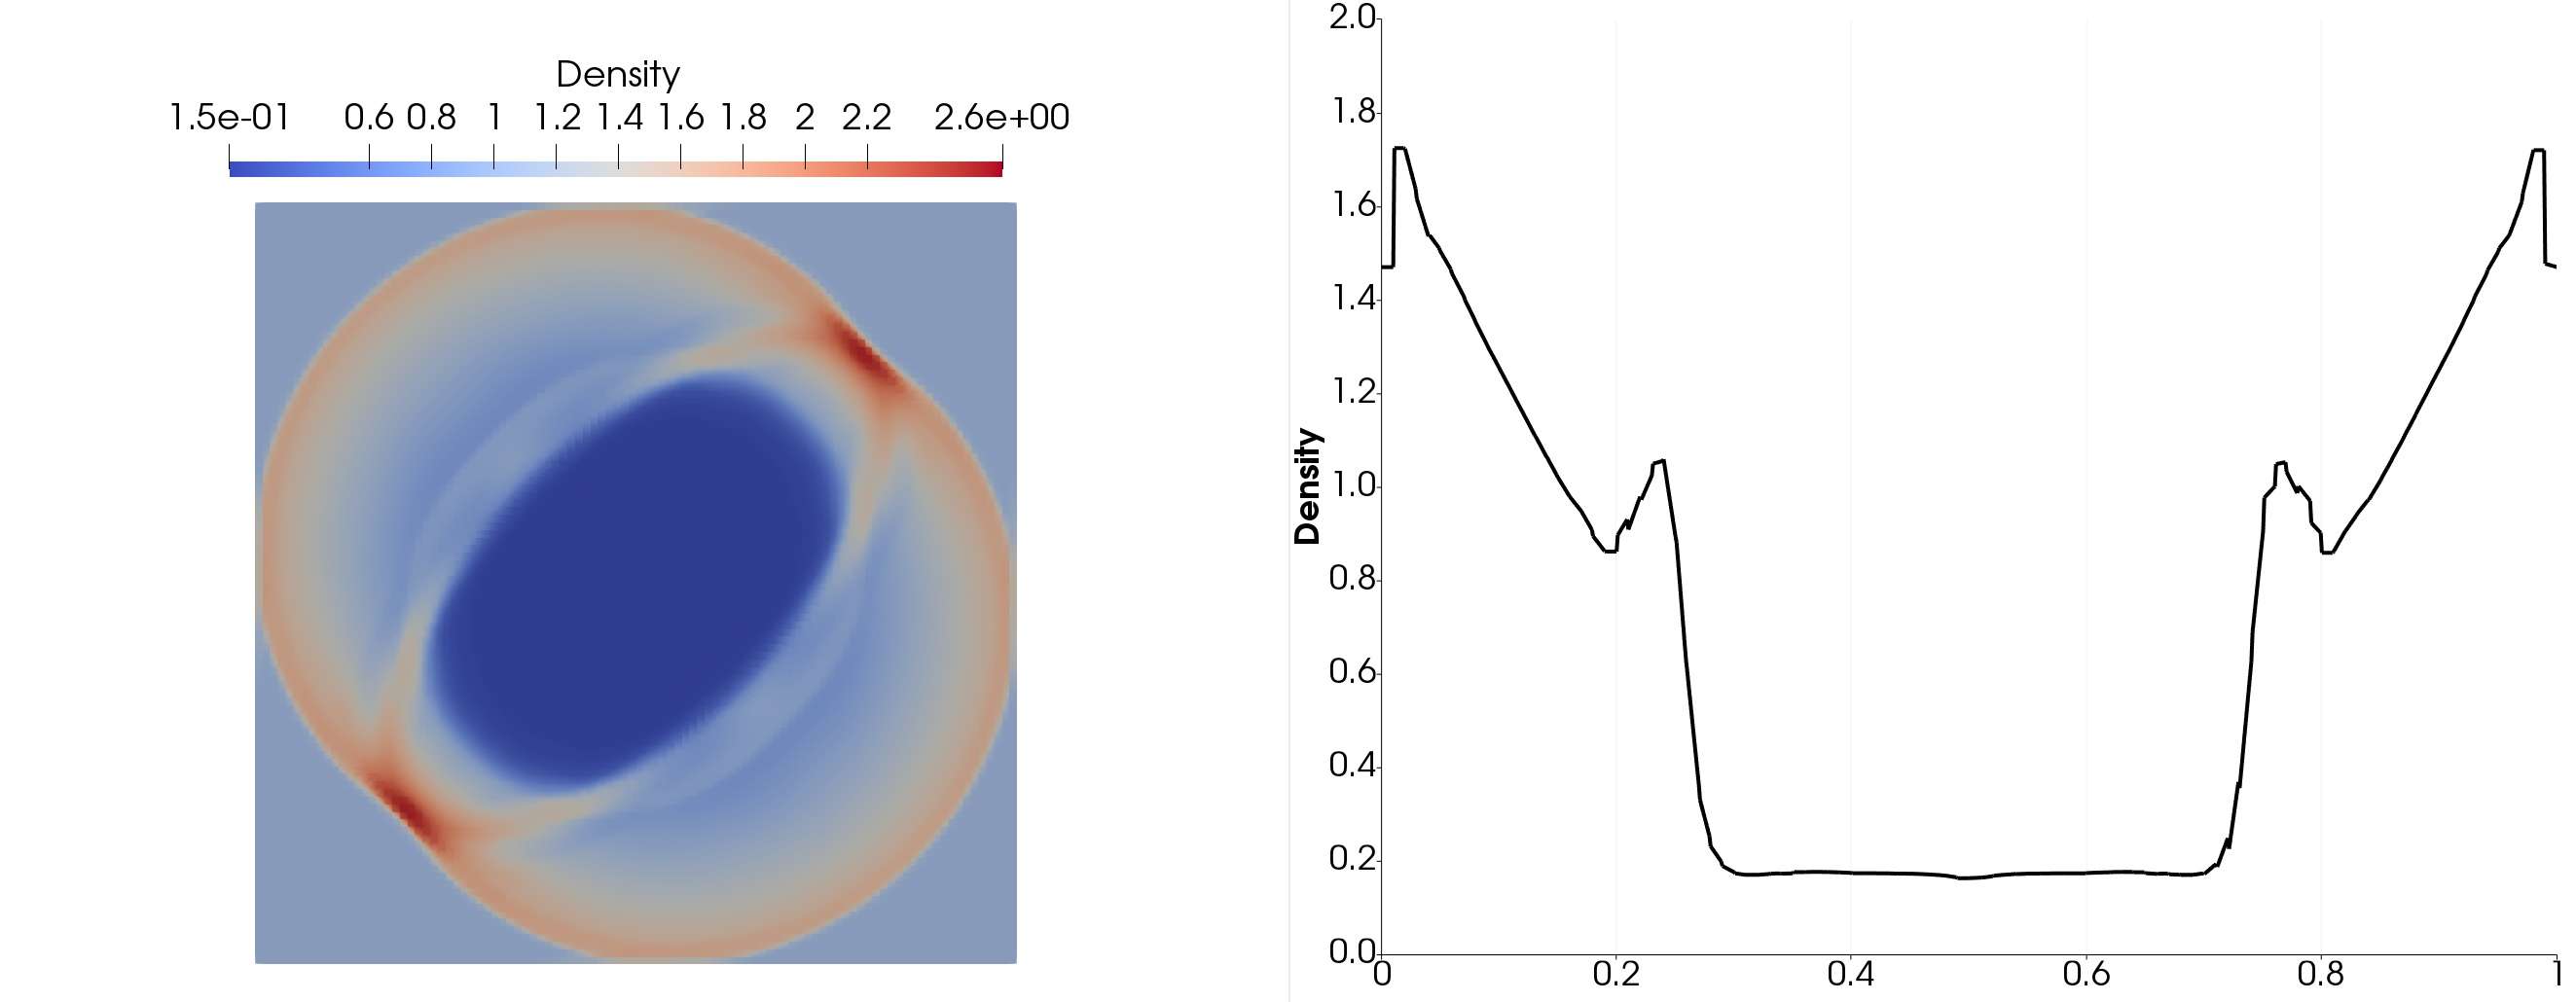
\includegraphics[width=\textwidth]{img/numflux/hl-1.jpg}
			\vspace{-3mm}
		\caption{Density at time $t = 0.2$, HLLD flux}
		\end{center}
		\label{numFluxCompare5}
	\end{figure}\vspace{-7mm}
	\newpage
	
	
	\begin{figure}[H]
		\begin{center}
			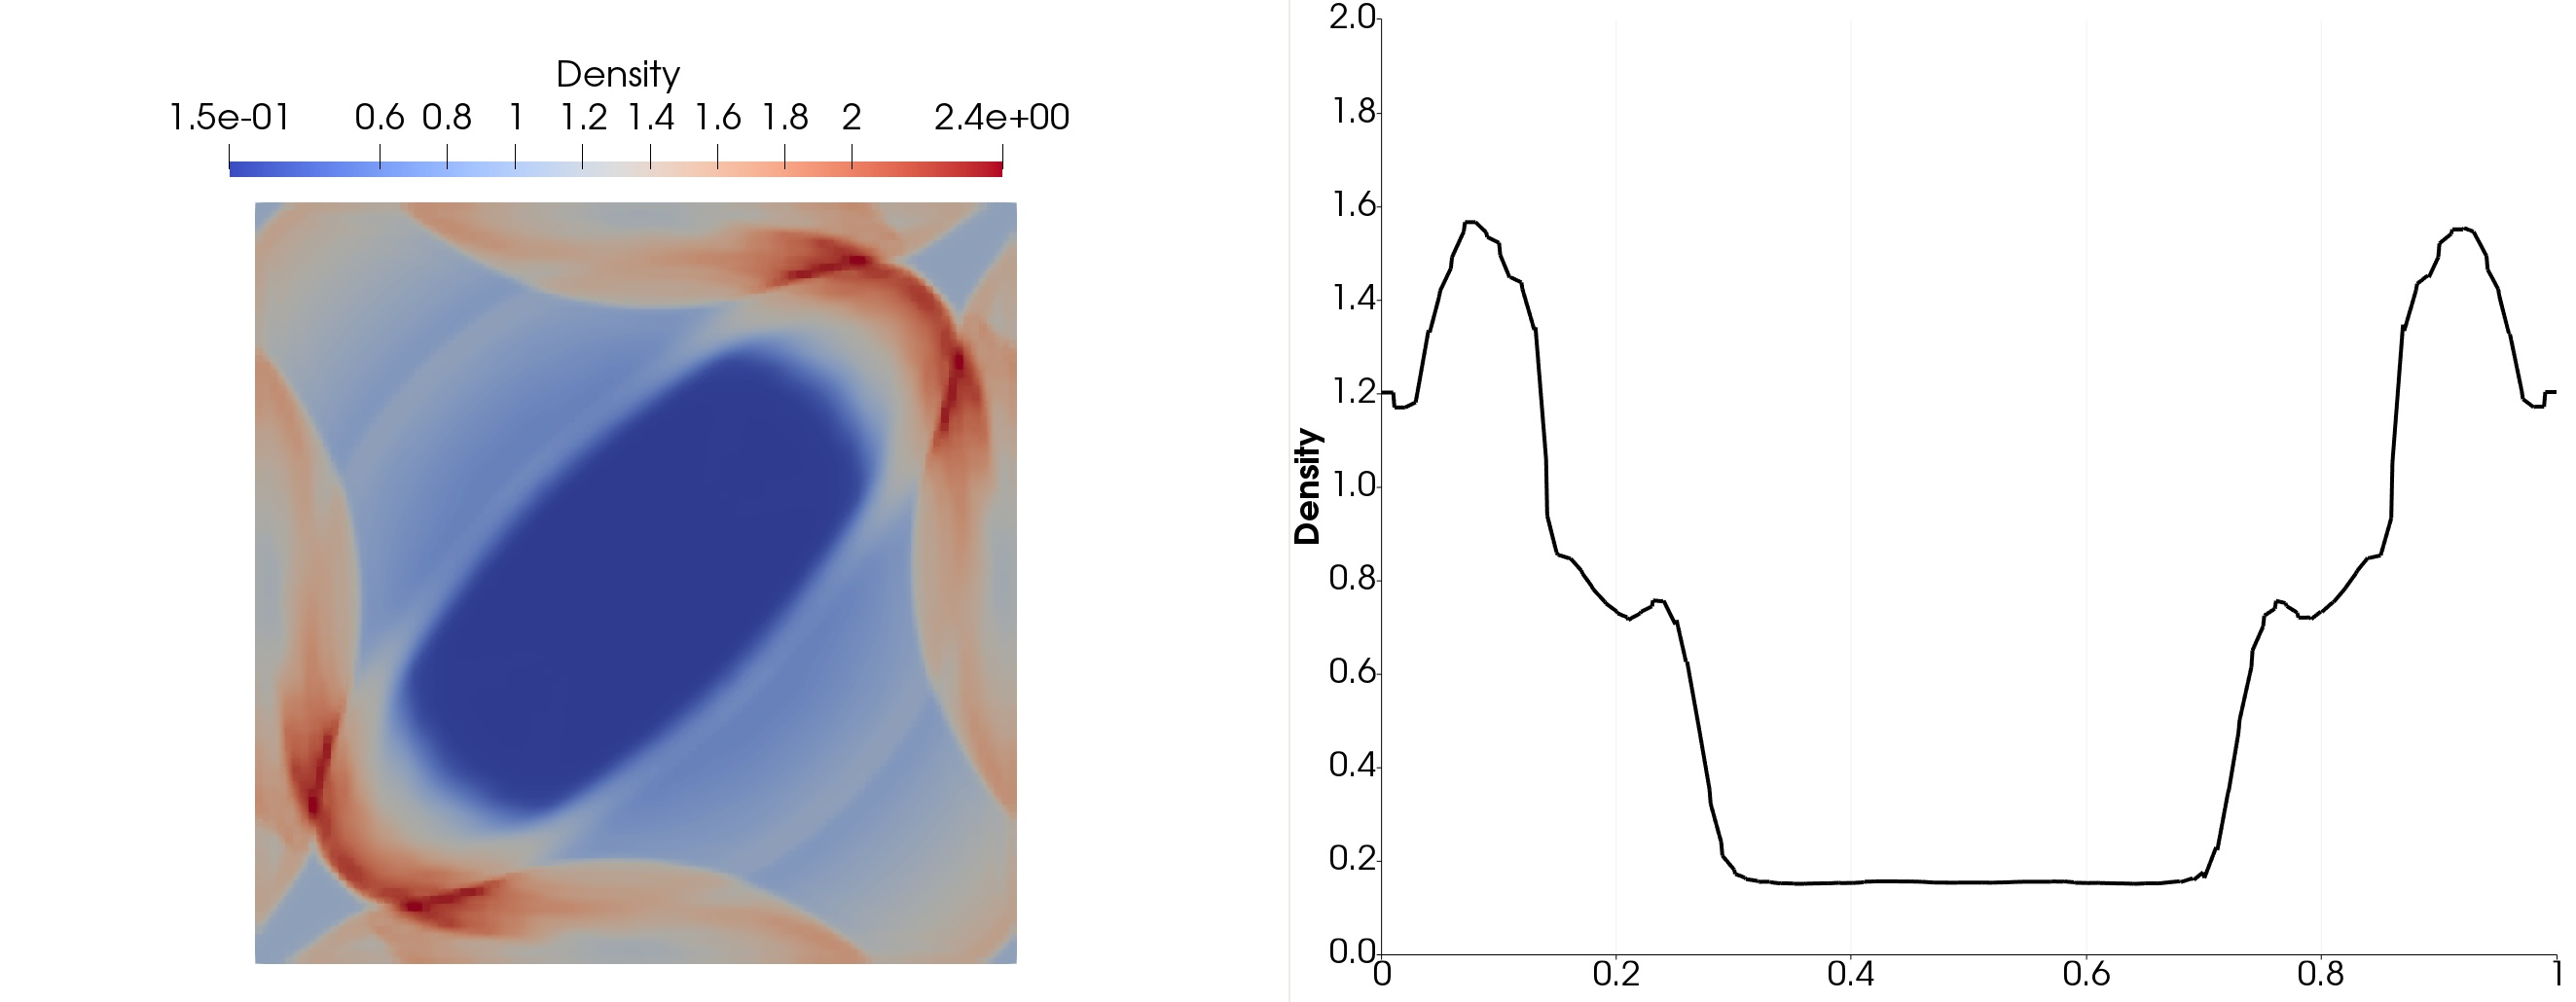
\includegraphics[width=\textwidth]{img/numflux/lf-05-2.jpg}
			\vspace{-3mm}
		\caption{Density at time $t = 0.3$, Lax-Friedrichs flux with $\alpha = 0.5$}
		\end{center}
		\label{numFluxCompare6}
	\end{figure}\vspace{-7mm}
	\begin{figure}[H]
		\begin{center}
			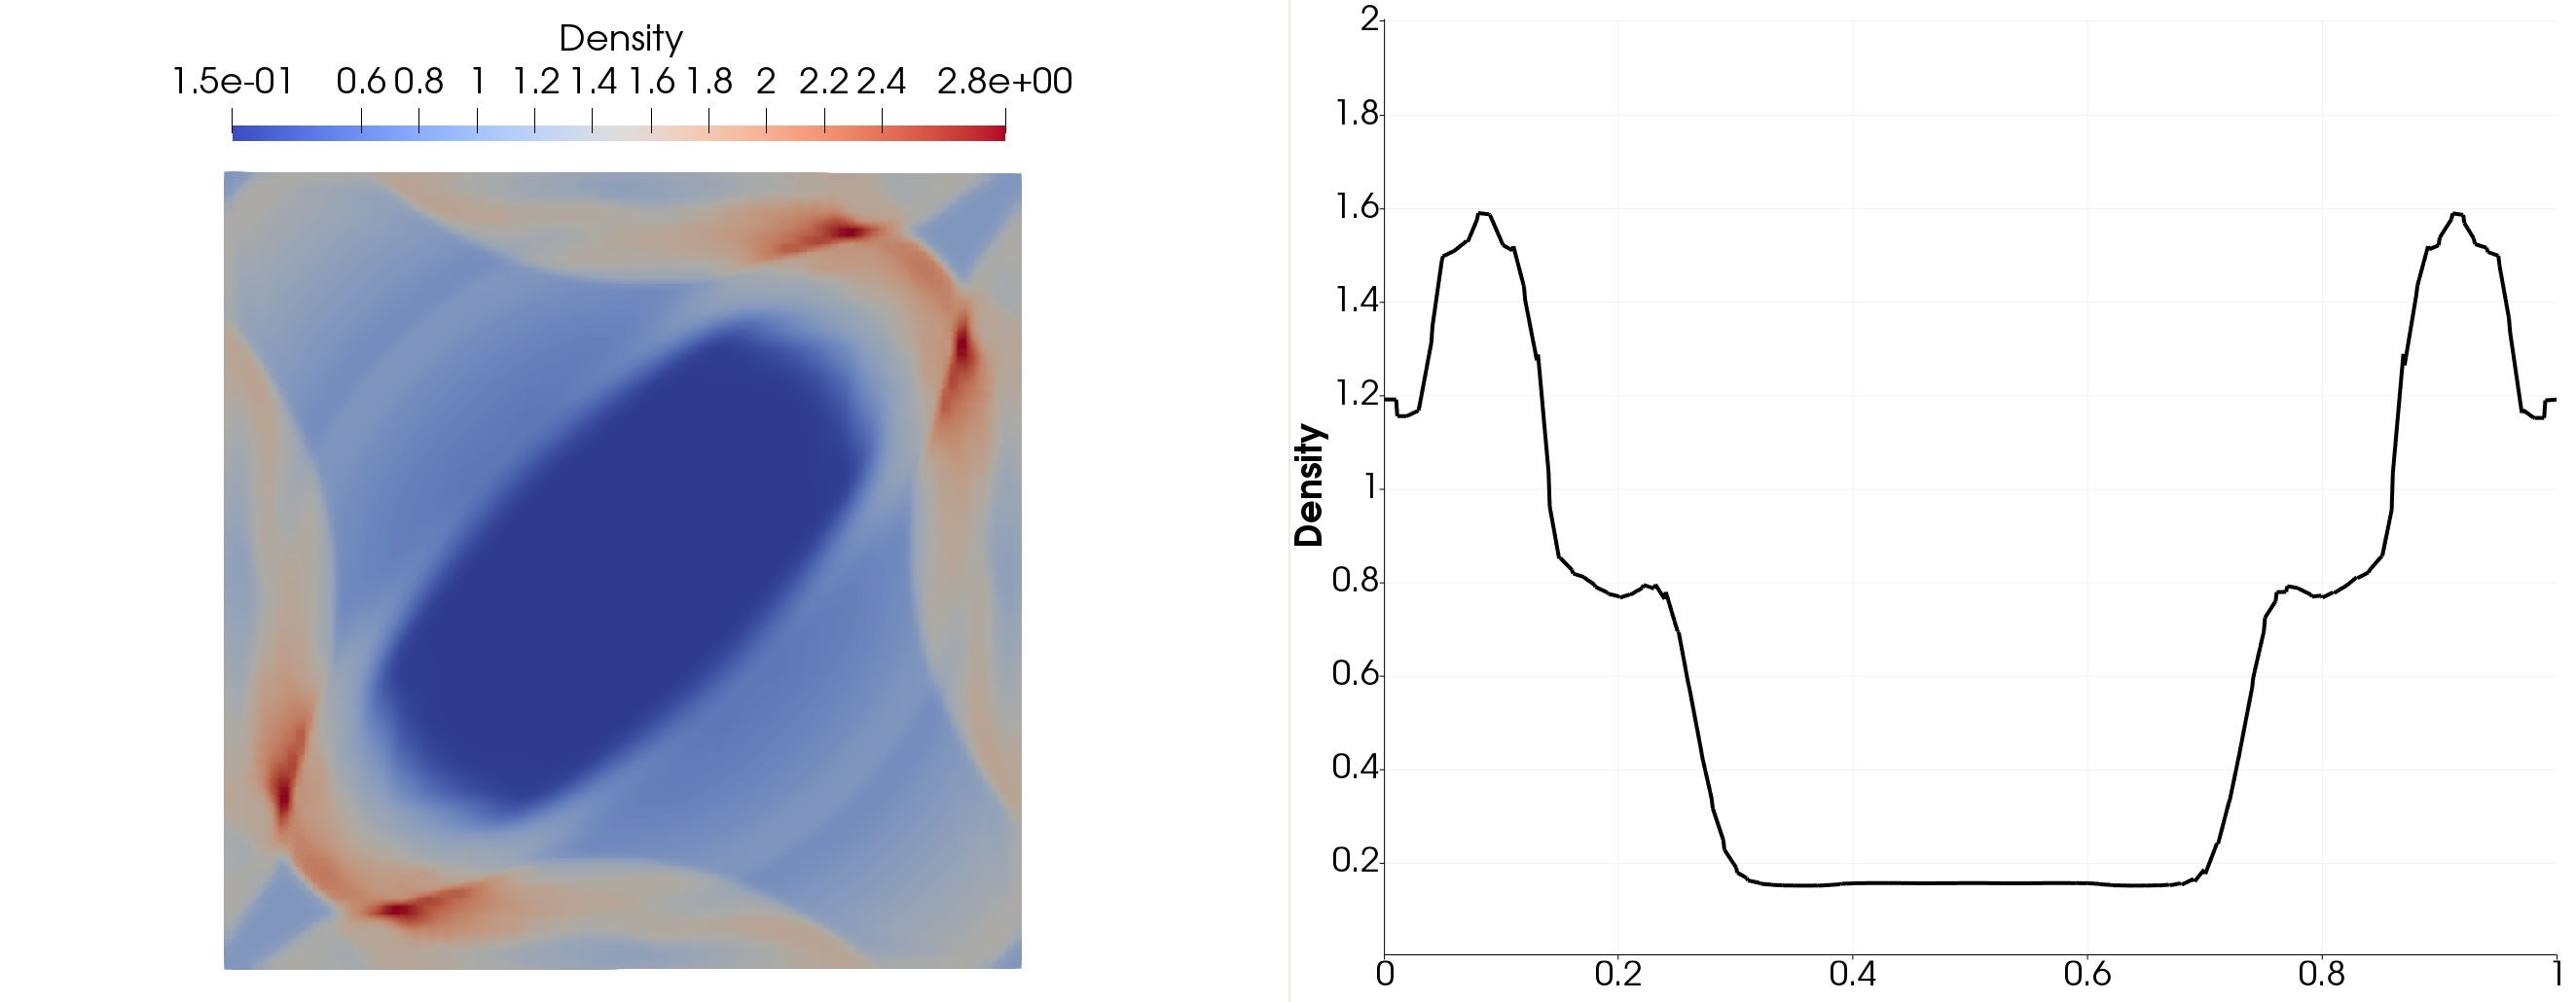
\includegraphics[width=\textwidth]{img/numflux/lf-10-2.jpg}
			\vspace{-3mm}
		\caption{Density at time $t = 0.3$, Lax-Friedrichs flux with $\alpha = 1.2$}
		\end{center}
		\label{numFluxCompare7}
	\end{figure}\vspace{-7mm}
	\begin{figure}[H]
		\begin{center}
			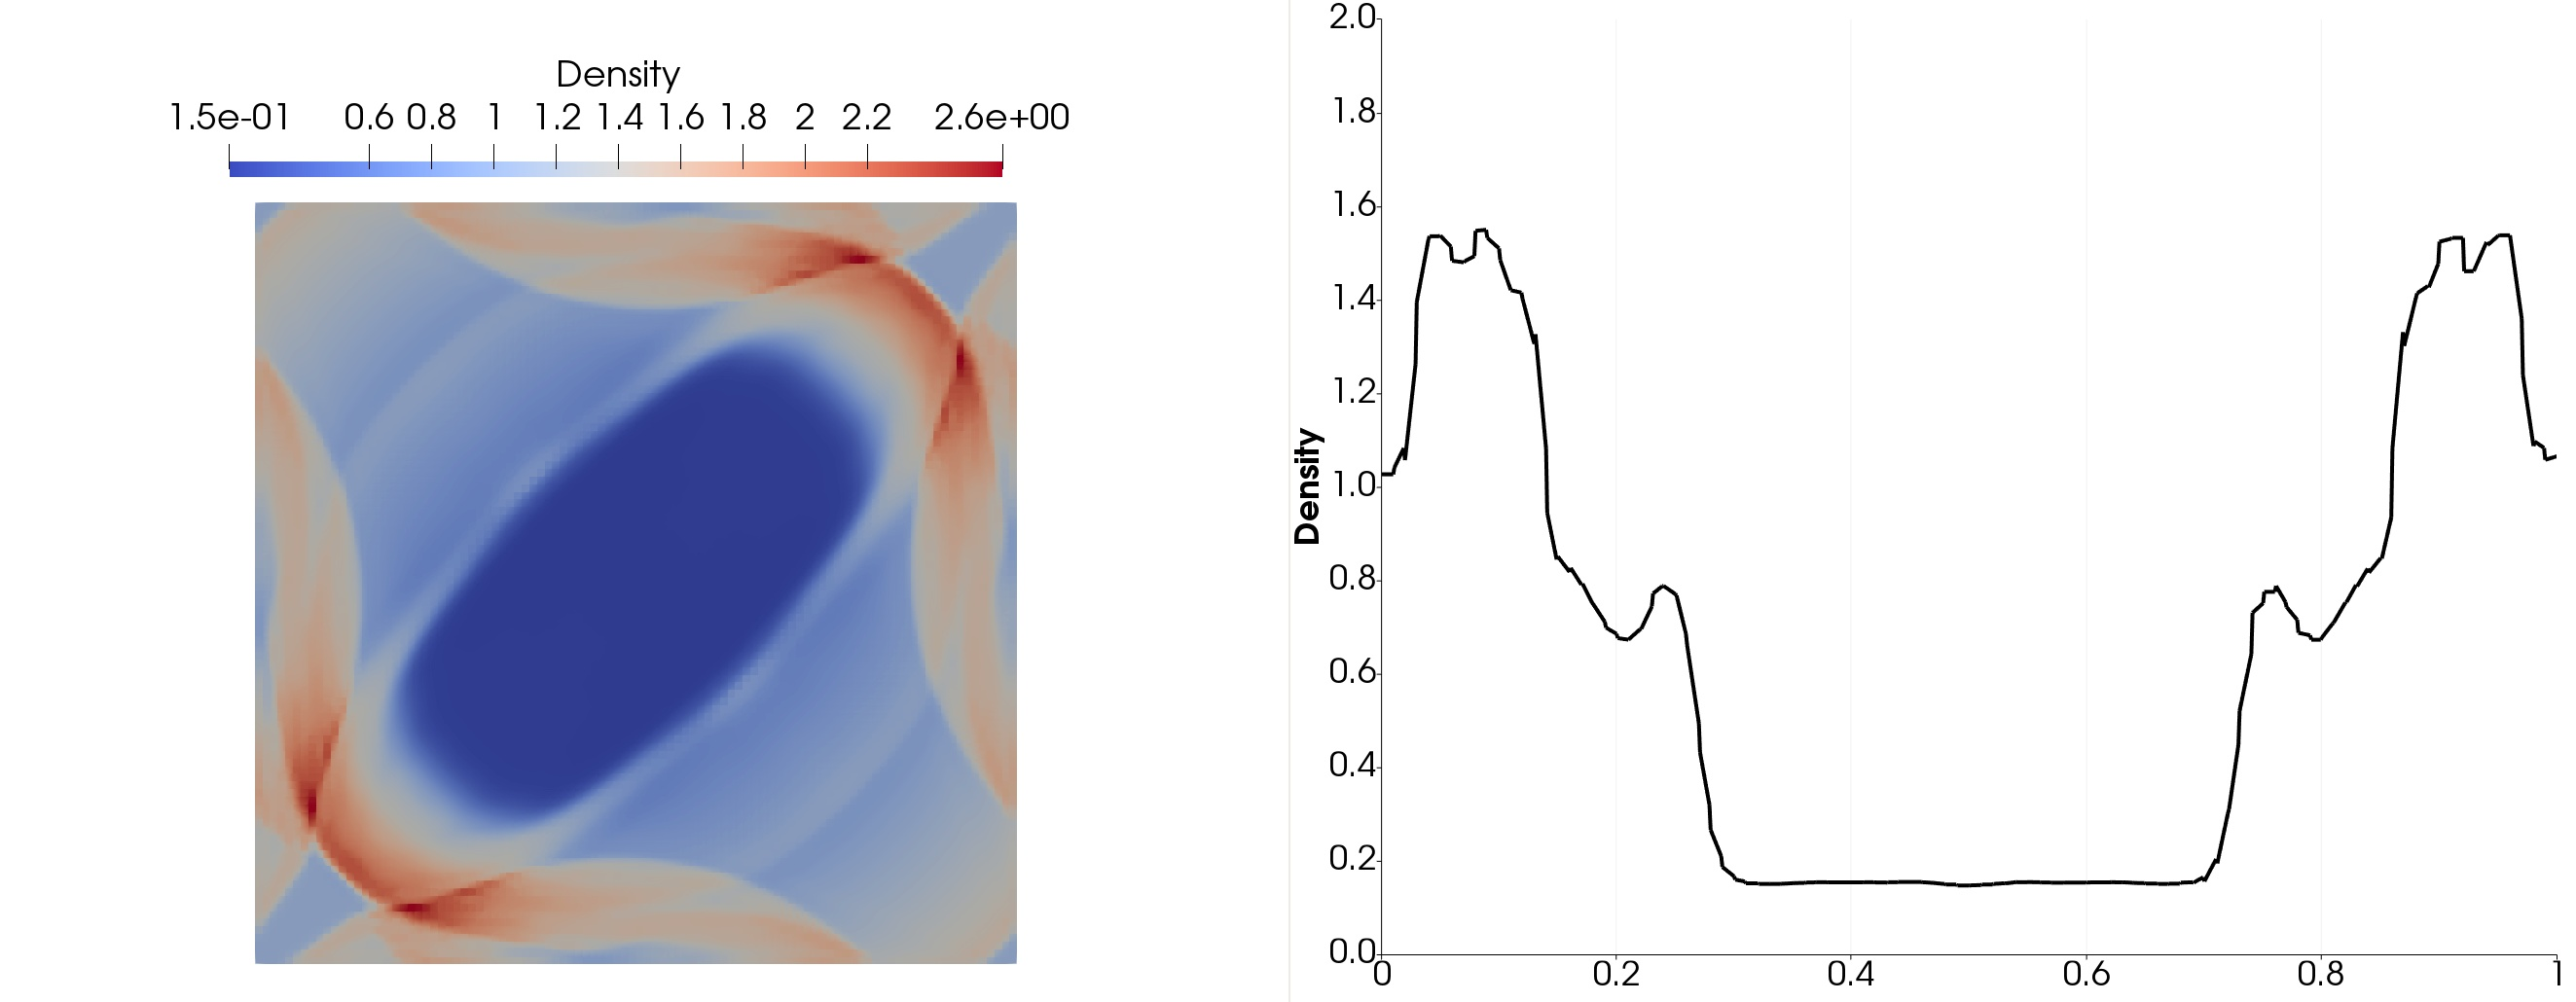
\includegraphics[width=\textwidth]{img/numflux/hl-2.jpg}
			\vspace{-3mm}
		\caption{Density at time $t = 0.3$, HLLD flux}
		\end{center}
		\label{numFluxCompare8}
	\end{figure}\vspace{-7mm}
	\newpage
	
There are a few observations from all the triplets of Figures:
\begin{itemize}
\item The Lax-Friedrichs flux is very sensitive to the choice of $\alpha$, for $\alpha = 1.2$, the solution is too diffusive,
\item The 'ideal' Lax-Friedrichs flux where $\alpha = 0.5$ is quantitatively and qualitatively very close to the HLLD flux.
\end{itemize}
The second observation could lead us to the conclusion that the Lax-Friedrichs flux, being simple to implement, is superior to HLLD which is quite complex. Unfortunately, as shown e.g. in \cite{lfunstable}, the Lax-Friedrichs flux is not stable enough to be used for arbitrary problem setup, also when handling solution with discontinuities, it is very dissipative \cite{lfdisc}.

Second reason why for practical usage of the developed code, the HLLD flux is strongly recommended is, that it is parameter-free, as opposed to Lax-Friedrichs flux having the stabilization parameter $\alpha$ which makes it performing differently for different problems, as per the value of $\alpha$.

\subsection{Numerical handling of boundary conditions}
In what follows, we are interested in using flux-induced inflow and outflow boundary conditions (see Section \cref{section:bcs}). Periodic boundary conditions are considered to be merely a special case of handling numerical fluxes across internal faces in $\Gamma_I$ .
To account for these boundary conditions, we need to investigate the term
$$
\int_{\Gamma_{ij}} \mrH\lo{\mrPsi_h}|_{ij}, {\mrPsi_h}|_{ji}, \bfn_{ij}\ro \mrvh
$$
for $\Gamma_{ij} \in \Gamma_B$ (see \cref{BndEdges}).
This term is used in \cref{DG2} for faces in $\Gamma_I$ which are internal and always have 2 values connected to them - $\mrPsi_h|_{ij}, {\mrPsi_h}|_{ji}$ - which induces the notation. On a boundary face, the corresponding value to ${\mrPsi_h}|_{ij}$ can be defined in the same way as in the case of $\Gamma_I$, but ${\mrPsi_h}|_{ji}$ needs to be defined.
\subsubsection{Inflow boundary condition}
First, if we want to prescribe an inflow boundary condition (i.e. we know what values should the state vector $\mrPsi_h$ have on ${\Gamma_{ij}}\in\Gamma_B$), we define
\be
\label{BC1} \overline{{\mrPsi_h}|_{ji}}
\ee
to be the prescribed value.

\subsubsection{Outflow boundary condition}
If we want to model an outflow boundary condition (i.e. do nothing condition), we may use the \textit{consistency} of the numerical flux $\mrH$ defined in \cref{FluxConsistent}, and define
\be
\label{BC2} \overline{{\mrPsi_h}|_{ji}} = {\mrPsi_h}|_{ij},
\ee
which is a suitable definition for the outflow boundary condition. It is important to mention, that setting the inflow boundary condition does not imply that solution values on this boundary equal to these prescribed value. This follows from the definition of broken Sobolev space (\cref{BrokenSobolev}). Moreover the values of the solution on the boundary also depend on the numerical flux used, as the values on the boundary are merely one of the input parameters for the flux (See \cref{NumFluxDef}).

\subsubsection{Periodic boundary conditions}
\label{sec:periodicDg}
Periodic boundary conditions come in the form described in \cref{periodicBCs}, for pair of points on the boundary (\cref{periodicMapping}). The point mapping is the main complication encountered, namely in the distributed computations, and moreover if AMR is used in distributed computations (see \cref{amrPer}). Otherwise, from the integral evaluation perspective, an face on a periodic boundary is approached in the very same way as internal faces (we have values from both sides, and we evaluate the numerical flux in quadrature points).

\subsubsection{DG full problem statement}
Now, taking \cref{BC1} and \cref{BC2}, we can enhance \cref{DG2} with an additional term, that will add the boundary conditions into the equation:
$$
\sum_{\Gamma_{ij}\in\Gamma_B} \int_{\Gamma_{ij}} \mrH\lo{\mrPsi_h}|_{ij}, \overline{{\mrPsi_h}|_{ji}}, \bfn_{ij}\ro \mrvh,
$$
so that the complete semi-discrete problem reads:
\begin{align}
\label{DG3} \int_{\Omega_{t}} \pds{{\mrPsi_h}}{t} \mrvh & -  \sum_{K^i \in T_h}\int_{K^i}\mrF\lo{\mrPsi_h}\ro \lo\nabla \cdot \mrvh\ro\\ \nonumber & + \sum_{\Gamma_{ij}\in\Gamma_I} \int_{\Gamma_{ij}} \mrH\lo{\mrPsi_h}|_{ij}, {\mrPsi_h}|_{ji}, \bfn_{ij}\ro \mrvh\\
\nonumber & + \sum_{\Gamma_{ij}\in\Gamma_B} \int_{\Gamma_{ij}} \mrH\lo{\mrPsi_h}|_{ij}, \overline{{\mrPsi_h}|_{ji}}, \bfn_{ij}\ro \mrvh\\
\nonumber & = \int_{\Omega_{t}} \mrS \mrvh.
\end{align}

\paragraph{}
Now we can formulate the definition of the \textit{semi-discrete solution ${\mrPsi_h} = {\mrPsi_h}\lo(t, \bfx\ro)$ of MHD equations \cref{conservativeGeneric}} as
\begin{enumerate}
    \label{discreteSlnDef}
    \item ${\mrPsi_h} \in C^{1}\lo\lo0, T\ro, \left[V_h\right]^8\ro$,
    \item \cref{DG3} holds for all $t\in\lo0, T\ro$, and all $\mrv\in \left[V_h\right]^8$,
    \item ${\mrPsi_h}\lo0, \bfx\ro = \Pi_h \mrPsi^0\lo\bfx\ro$,
\end{enumerate}
where $\Pi_h$ is a projection of the initial condition $\mrPsi^0$ onto $\left[V_h\right]^8$.


